%% TrustTier -- CSD436 Blockchain Technology, final project paper
%% Two-column ACM format (acmart, sigconf). Compile with pdfLaTeX + BibTeX (Overleaf: default settings).
\documentclass[sigconf,nonacm]{acmart}

\usepackage{tikz}
\usetikzlibrary{positioning,arrows.meta,fit,backgrounds,calc,shapes.geometric}
\usepackage{pgfplots}
\pgfplotsset{compat=1.17}
\usepackage{booktabs}
\usepackage{tabularx}
\usepackage{multirow}
\usepackage{enumitem}
\usepackage{amsmath}

\newcommand{\code}[1]{\texttt{\small #1}}
\newcolumntype{L}{>{\raggedright\arraybackslash}X}
\newcolumntype{P}[1]{>{\raggedright\arraybackslash}p{#1}}
\setlist{leftmargin=*,itemsep=1pt,topsep=2pt}
\emergencystretch=2em

% One colour per tier, used in every figure
\definecolor{tierzero}{HTML}{2A9D8F}
\definecolor{tierone}{HTML}{E9A23B}
\definecolor{tiertwo}{HTML}{D1495B}
\definecolor{accent}{HTML}{2A78D6}
\definecolor{muted}{HTML}{6B6B6B}

\begin{document}
\sloppy

\title{TrustTier: Cost-Tiered Zero-Knowledge Verification of DeFi Liquidation Decisions on Verified On-Chain Inputs}
\subtitle{CSD436 Blockchain Technology --- Final Project Paper}

\author{Gaurav Rai}
\affiliation{%
  \institution{Shiv Nadar University}
  \city{Delhi NCR}
  \country{India}}
\email{2410110133}

\author{Shaurya Sharma}
\affiliation{%
  \institution{Shiv Nadar University}
  \city{Delhi NCR}
  \country{India}}
\email{2410110317}

\author{Sharanya Gupta}
\affiliation{%
  \institution{Shiv Nadar University}
  \city{Delhi NCR}
  \country{India}}
\email{2410110315}

\renewcommand{\shortauthors}{Rai, Sharma and Gupta}

\begin{abstract}
Lending protocols liquidate a borrower only once the loan-to-value ratio (LTV) crosses a threshold, which is free to check but acts too late in a crash; acting earlier needs a risk model, and a model's score is usually computed by an operator nobody can audit. Zero-knowledge machine learning (zkML) can prove that a score came from a committed model, but a proof-verified decision costs about 0.9\,M gas, too much to spend on every position. TrustTier makes the strength of verification grow with risk. A position far from its liquidation boundary may be decided by a bonded heuristic claim (Tier~0), one approaching it by a bonded, salted commitment to a registered model's output (Tier~1), and one at the boundary only by an on-chain-verified Halo2 zk-SNARK of the model's inference (Tier~2). Cheap claims stay accountable through a one-hour window in which anyone can slash a false claim with a Tier-2 proof; the bond scales with the base fee so that slashing always pays, challenges are committed before they are revealed so they cannot be front-run, and a Tier-1 claimant must open its commitment or forfeit. A verified Tier-2 approval is the only way the lending protocol's liquidator can execute a (soft) liquidation, once, within 30 minutes.

A tiered design is only as honest as whoever picks the tier and supplies the model's inputs. TrustTier therefore trusts neither: the contract reads every input itself from the lending protocol and Chainlink-style feeds, computes the distance $\delta$ to the boundary, refuses a tier too weak for it, and accepts a proof only if its public inputs equal the features it computed in the same transaction. Cheap claims snapshot their features, so a challenge is judged on the facts at claim time.

The prototype comprises nine Solidity contracts (including the liquidator that consumes approvals, an Aave~V3 adapter and multisig-plus-timelock governance), a router, an EZKL proving pipeline, a sentinel and a wallet-signed DApp that also runs as an in-browser simulation; 126 contract tests and 82 Python tests pass. On 374 positions (74 real Aave~V2 snapshots and 300 synthetic), tiering costs 210.3\,M gas against 328.4\,M for always proving, a 36.0\% saving; a sweep of 34 band settings shows the deployed bands are Pareto-optimal. In a 30-day stress test of 3,000 positions on identical price paths, acting on the proven model cuts forced liquidations by 88\% and insolvencies from 61 to 2 compared with the health-factor rule, at the price of decision gas and 26\% unnecessary soft liquidations; the gas makes daily monitoring affordable for retail positions on a rollup, not on L1. Opcode traces of whole blocks show that 374 decisions parallelize to 15.3$\times$ on 16 threads, that bonds paid as \code{msg.value} would cap this at 3.35$\times$ on engines that treat balance updates as read-modify-writes, and that deposit-funded bonds remove that bottleneck.
\end{abstract}

\keywords{DeFi, liquidations, zkML, zk-SNARK, EZKL, Halo2, smart contracts, optimistic verification, oracles, parallel execution}

\maketitle

%% ===================================================================
\section{Introduction}

Lending protocols such as Aave, Compound and MakerDAO hold billions of dollars of collateral, and a liquidation sells part of it at a discount. In the four largest protocols, 28,138 liquidations sold USD~807.46\,M of collateral~\cite{qin2021liquidations}. Whether a position is truly at risk is increasingly judged by a model that looks beyond the LTV, at volatility, price momentum and account history. Today that model runs on an operator's server. Borrowers, liquidators and auditors see only the outcome, and must trust that the score came from the claimed model, on the real inputs, and that neither the model nor the record was quietly changed.

\paragraph{Why a model at all.} Every protocol already has a free, deterministic rule: liquidate once LTV reaches the threshold (Aave's health factor below 1). It acts only at the boundary, so a crash day can carry a position from safe to under water before any keeper moves, and the protocol absorbs bad debt. A model that sees volatility and momentum can act \emph{before} the boundary with a smaller, \emph{soft} liquidation. That is only acceptable if the model's verdict is verifiable, and only affordable if verification is not paid on every position. Section~\ref{sec:eval-hf} measures this trade against the health-factor rule on identical price paths.

Recent work shows that such decisions \emph{can} be verified on-chain, either by running a small model inside a contract~\cite{alhaidari2025onchain} or by verifying a zk-SNARK of its inference~\cite{chen2024zkml,kang2022scaling}. The obstacle is cost. In our implementation a proof-verified liquidation decision costs 878,059 gas and about 16\,s of proving, 3.3 times a bonded heuristic decision. Spending that on every position is wasteful, because most positions are nowhere near their liquidation boundary.

\paragraph{The idea.} TrustTier spends verification where it matters. It borrows the intuition of memory tiering, where hot data gets the expensive fast tier: positions far from the boundary get cheap, bonded claims, and only positions at the boundary must carry a zero-knowledge proof. The cheap tiers are optimistic, as in optimistic rollups~\cite{kalodner2018arbitrum} and optimistic ML~\cite{conway2024opml}, but a dispute is settled by a single zk-SNARK rather than an interactive bisection game.

\paragraph{The catch, and our answer.} Tiering creates a new trust problem. Our midterm prototype let an off-chain router compute $\delta$ and choose the tier, and a later version let a ``feature oracle'' commit each position's inputs. A reviewer put the problem precisely: \emph{the router is an unaudited operator, and the chain cannot check $\delta$}. Whoever supplies the inputs controls which tier applies and what the proof proves. This paper's central design change removes that party entirely. The contract reads collateral, debt and the liquidation threshold from the lending protocol, volatility and 24-hour momentum from Chainlink feeds, and account history from protocol timestamps; it quantizes them exactly as the circuit does, enforces the tier from its own $\delta$, and requires the proof's public inputs to equal its own features. We call this \emph{verified inputs instead of trusted inputs}.

\paragraph{Contributions.}
\begin{itemize}
  \item A risk-proportional verification scheme with three tiers whose boundaries are enforced \emph{on-chain}, from inputs the contract reads itself (Sections~\ref{sec:design-tiers}--\ref{sec:design-inputs}).
  \item A bonded challenge window with feature snapshots, a precise position lifecycle in which a Tier-2 proof supersedes any pending cheap claim, and deposit-funded bonds (Sections~\ref{sec:design-challenge}--\ref{sec:design-concurrency}).
  \item An incentive and execution layer: gas-scaled bonds that make slashing profitable at any gas price, a protocol-funded reward pool for honest claims, Tier-1 commitments that must be opened, commit-reveal challenges, feature anchors for slow proofs, and a liquidator contract that executes each Tier-2 approval exactly once (Sections~\ref{sec:design-incentives}--\ref{sec:design-consumer}).
  \item A complete implementation: nine contracts, an EZKL/Halo2 circuit with a 15.6\,KB verifier, an Aave~V3 adapter, multisig-plus-timelock governance, a router, a sentinel and a DApp (Section~\ref{sec:impl}).
  \item An evaluation with real proofs and measured gas: a comparison with the health-factor rule on identical price paths, the economics of the challenge game and of deployment on L1 versus a rollup, an outcome-labelled test on real Aave data, tiering cost, ablations of every design component, a 34-point band sweep, a threshold sweep, model calibration, and three concurrency studies (modelled scheduling, opcode-traced blocks executed on 1--64 simulated threads, and competing liquidator threads on a live node) (Section~\ref{sec:eval}).
  \item A security analysis of 29 findings, each with its status (Section~\ref{sec:security}).
\end{itemize}

\paragraph{Scope.} TrustTier governs the \emph{decision} that a liquidation is justified and gates its execution: in the demo lending pool, only \code{TrustTierLiquidator}, and only on an open Tier-2 approval, can liquidate. It does not replace a protocol's own health-factor liquidations, which remain the fallback. The prototype runs on a local Ethereum chain (Hardhat) with a tested deployment path to the Sepolia testnet.

%% ===================================================================
\section{Background and Motivation}
\label{sec:background}

\paragraph{Liquidations.} A lending position is liquidatable when its LTV exceeds the market's liquidation threshold $\theta$. Liquidation designs regularly sell more collateral than needed; Aave~V2 had accumulated up to USD~87.4\,K of bad debt by April 2021; and 73.97\% of liquidations paid an above-average transaction fee because liquidator bots race each other~\cite{qin2021liquidations}. Small price moves can make large volumes of positions liquidatable at once~\cite{perez2021knife}. Decisions near the boundary are therefore both the most contested and the most consequential.

\paragraph{zkML.} A zk-SNARK lets a prover convince a verifier that a computation produced an output without revealing private inputs~\cite{groth2016size,gabizon2019plonk}. EZKL~\cite{ezkl} compiles an ONNX model into a Halo2 (PLONKish) circuit with KZG polynomial commitments~\cite{kate2010kzg} and emits a Solidity verifier; the proof is small and checked by a pairing computation. Proving cost grows with model size~\cite{peng2025survey,chen2024zkml}, which is why TrustTier uses a deliberately small 5$\to$8$\to$1 network.

\paragraph{Three observations.} (1) \emph{Risk is concentrated}: in our 374-position evaluation set only 144 positions (38.5\%) are within $\delta\le0.05$ of their threshold, so proving every position wastes most of the cost. (2) \emph{Blockchains already provide the right primitives}: immutable logs give non-repudiation, consensus order resolves races between bots, contract-held bonds make cheap claims costly to fake, and Chainlink-style feeds and protocol state are readable on-chain, so inputs need not be trusted. (3) \emph{Liquidations come in bursts}: when prices fall, many positions cross the boundary within the same few blocks, so the contracts should not stop a parallel execution engine from processing those decisions concurrently~\cite{gelashvili2023blockstm}.

%% ===================================================================
\section{Related Work}
\label{sec:related}

Prior work verifies ML decisions on-chain either completely, running or proving every inference, or optimistically, checking only disputes. None adapts the strength of verification to the risk of the individual decision, and none removes trust in the inputs of a tiered scheme. Table~\ref{tab:lit} compares the closest work.

\begin{table*}[t]
  \caption{Verifiable and on-chain ML: what each work does and the gap TrustTier addresses.}
  \label{tab:lit}
  \small
  \begin{tabularx}{\textwidth}{@{}P{3.3cm}LLLL@{}}
    \toprule
    \textbf{Work} & \textbf{Problem} & \textbf{Approach} & \textbf{Key result} & \textbf{Gap TrustTier addresses} \\
    \midrule
    Alhaidari et al., AFT 2025~\cite{alhaidari2025onchain} (primary baseline) & Off-chain detectors miss DeFi exploits executed within one block & Train models on Layer~2 under a Proof-of-Improvement protocol; run quantized models directly in an L1 contract & Over 97\% detection on 298 real exploits; 57,603--506,397 gas per inference & Weights and inputs become public; TrustTier keeps the model private, proves only where needed, and verifies its inputs on-chain \\
    \addlinespace
    Chen et al., EuroSys 2024~\cite{chen2024zkml}; Kang et al., 2022~\cite{kang2022scaling} & Zero-knowledge proofs of ML inference are slow & Compile ML models to optimized Halo2 circuits & Practical proofs for realistic models; cost grows with model size & A proof on every decision is still costly; TrustTier proves only near the boundary \\
    \addlinespace
    Garg et al., CCS 2023~\cite{garg2023zkpot} & Proving how a model was trained & Zero-knowledge proofs of training & Feasible for simple models such as logistic regression & Model provenance can be proved; TrustTier binds every decision to a registered model hash \\
    \addlinespace
    Peng et al., 2025~\cite{peng2025survey} & Fragmented landscape of verifiable ML & Survey of ZKP-based verifiable training, inference and testing & Proving cost is the main barrier & Justifies the deliberately tiny model \\
    \addlinespace
    Conway et al., 2024~\cite{conway2024opml}; Kalodner et al., 2018~\cite{kalodner2018arbitrum} & Full verification is too heavy & Optimistic execution: results accepted unless disputed via interactive bisection & Low cost; finality after a challenge period & TrustTier keeps the bonded window but settles disputes with one zk-SNARK, judged on an on-chain feature snapshot \\
    \bottomrule
  \end{tabularx}
\end{table*}

\paragraph{DeFi liquidations and attacks.} Qin et al.~\cite{qin2021liquidations} and Perez et al.~\cite{perez2021knife} measure liquidation incentives, over-liquidation and instability. Zhou et al.~\cite{zhou2023sok} catalogue DeFi attacks, including oracle manipulation, which in TrustTier could move a position between tiers; we therefore add staleness checks and leave manipulation resistance to the oracle (Section~\ref{sec:limits}). Daian et al.~\cite{daian2020flashboys} and Qin, Zhou and Gervais~\cite{qin2022bev} show that the public mempool lets bots front-run and reorder transactions, so liquidators race for the same position. TrustTier admits one decision per position and makes losing attempts revert cheaply (Section~\ref{sec:eval-race}).

\paragraph{Concurrent execution of smart contracts.} Dickerson et al.~\cite{dickerson2017adding} introduced speculative execution by miners, who publish a schedule that validators replay. Anjana et al.~\cite{anjana2019efficient} execute a block with optimistic software transactional memory and ship a block graph for parallel validation; OptSmart~\cite{anjana2022optsmart} reduces its space cost. Saraph and Herlihy~\cite{saraph2020empirical} measured on historical Ethereum blocks how much speculative execution helps, and found that conflicts concentrate on a small amount of popular state. Block-STM~\cite{gelashvili2023blockstm} runs in production with multi-version memory and a preset order, ParallelEVM~\cite{lin2025parallelevm} detects conflicts at the level of individual operations, and Conthereum~\cite{chahoki2025conthereum} schedules conflicting transactions in advance. All of them gain only when transactions touch disjoint state, which is why TrustTier keys every write by position, account or model, and why we trace real read/write sets rather than assume them.

\paragraph{Contract security and proof systems.} Atzei et al.~\cite{atzei2017survey} classify attacks on Ethereum contracts, including reentrancy and failed sends; TrustTier answers them with checks-effects-interactions and pull payments. KZG commitments~\cite{kate2010kzg} need a trusted setup; zk-STARKs~\cite{bensasson2019stark} remove it at the price of much larger proofs~\cite{nainwal2025comparative}, a trade-off Section~\ref{sec:design-stark} quantifies.

%% ===================================================================
\section{Threat Model and Goals}
\label{sec:threat}

\paragraph{Actors.} \emph{Borrowers} own positions in a lending protocol. \emph{Liquidators} (people or bots) submit decisions and may be dishonest: they may claim a cheaper tier than a position deserves, submit forged or replayed proofs, front-run each other, or try to lock a position to delay its liquidation. The \emph{router} is our reference liquidator and gets no special rights. \emph{Watchers} (any user of the DApp, or the sentinel) challenge false claims. \emph{Governance} is an M-of-N multisig behind a timelock.

\paragraph{Trust assumptions.} We trust exactly what the lending protocol already trusts: its own accounting (collateral, debt, threshold) and its price and volatility feeds, which must be fresh. We trust the soundness of Halo2 with KZG over BN254 under a correctly generated structured reference string (SRS), and that governance changes are visible a full delay before they apply. We do \emph{not} trust the router, any liquidator, or any off-chain computation of features or $\delta$.

\paragraph{Goals.}
\begin{description}[leftmargin=0pt,itemsep=2pt]
  \item[G1 Input integrity.] Every decision is made on features derived from on-chain state; no party can substitute its own.
  \item[G2 Tier soundness.] No decision uses a tier weaker than the position's on-chain $\delta$ allows.
  \item[G3 Proof binding.] A Tier-2 proof approves a liquidation only for the position, and the state, it was made on, and only if it proves high risk.
  \item[G4 Accountability.] A false cheap claim can be slashed; an honest one cannot.
  \item[G5 Liveness.] No claim can delay a needed liquidation, and no position can be locked forever.
  \item[G6 Exactly once.] Racing liquidators finalize a position at most once, and a race over one position never delays a decision about another.
  \item[G7 Governed change.] No single key can change what the system trusts.
  \item[G8 Incentive compatibility.] Slashing a false claim pays for itself at any gas price, a claimant cannot keep its committed score hidden, and a challenge seen in the mempool cannot be stolen.
\end{description}

%% ===================================================================
\section{Design}
\label{sec:design}

\subsection{Tiers}
\label{sec:design-tiers}

TrustTier sets the evidence a decision must carry by the position's distance from its boundary, $\delta = \theta - \mathrm{LTV}$, where $\theta$ is the position's own liquidation threshold (Figure~\ref{fig:bands}, Table~\ref{tab:tiers}). Tier~0 requires $\delta > B_0 = 0.15$, Tier~1 requires $\delta > B_1 = 0.05$, and Tier~2 is always allowed: a stronger tier than necessary is never refused. Section~\ref{sec:eval-bands} justifies both band values.

\begin{figure}[t]
  \centering
  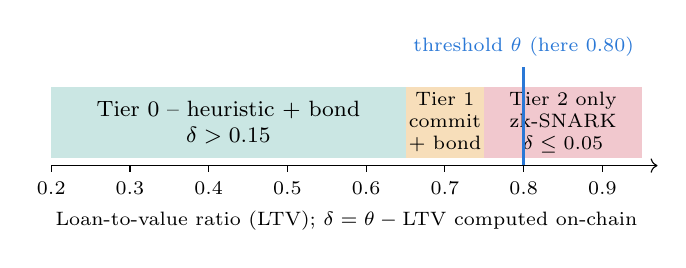
\begin{tikzpicture}[x=10cm,y=1cm,font=\footnotesize]
    \fill[tierzero!25] (0.20,0) rectangle (0.65,0.9);
    \fill[tierone!35]  (0.65,0) rectangle (0.75,0.9);
    \fill[tiertwo!30]  (0.75,0) rectangle (0.95,0.9);
    \node[align=center] at (0.425,0.45) {Tier 0 -- heuristic + bond\\$\delta>0.15$};
    \node[align=center,font=\scriptsize] at (0.70,0.45) {Tier 1\\commit\\+ bond};
    \node[align=center,font=\scriptsize] at (0.85,0.45) {Tier 2 only\\zk-SNARK\\$\delta\le0.05$};
    \draw[very thick,accent] (0.80,-0.1) -- (0.80,1.15) node[above,font=\scriptsize]{threshold $\theta$ (here 0.80)};
    \draw[->] (0.20,-0.1) -- (0.97,-0.1);
    \foreach \x in {0.2,0.3,...,0.91} \draw (\x,-0.1) -- (\x,-0.18) node[below,font=\scriptsize]{\pgfmathprintnumber[fixed,precision=1]{\x}};
    \node[below,font=\scriptsize] at (0.575,-0.55) {Loan-to-value ratio (LTV); $\delta=\theta-\mathrm{LTV}$ computed on-chain};
  \end{tikzpicture}
  \caption{Verification tiers as bands of LTV for a market with $\theta=0.80$. The contract reads $\theta$ per position and refuses a tier whose band the position is not in.}
  \label{fig:bands}
\end{figure}

\begin{table}[t]
  \caption{Tiers, what each puts on-chain, and measured gas per decision (full transaction, including reading the position, two feeds and the 24-hour price round). $^{*}$Claim 340,072 plus the mandatory reveal, 39,089.}
  \label{tab:tiers}
  \footnotesize
  \setlength{\tabcolsep}{3pt}
  \begin{tabularx}{\columnwidth}{@{}lP{1.15cm}Lr@{}}
    \toprule
    \textbf{Tier} & \textbf{Allowed} & \textbf{Evidence on-chain} & \textbf{Gas} \\
    \midrule
    0 Heuristic & $\delta>0.15$ & Decision record, feature snapshot, gas-scaled bond slashable for 1\,h & 269,534 \\
    1 Commitment & $\delta>0.05$ & Registered model, salted commitment to (features, score) that must be opened in the window, snapshot, same bond & 379,161$^{*}$ \\
    2 zk-SNARK & always & Halo2 proof that the model on the position's on-chain features outputs ``high risk''; approves one liquidation & 878,059 \\
    \bottomrule
  \end{tabularx}
\end{table}

\subsection{Verified inputs instead of trusted inputs}
\label{sec:design-inputs}

\paragraph{Where every feature comes from.} The engine's view function \code{currentFeatures(positionId, pastRoundId)} computes the model's five features from on-chain sources only (Table~\ref{tab:features}). Positions are read through a small interface, \code{IPositionSource}, which returns collateral and debt (USD with 8 decimals), the liquidation threshold, the opening and last top-up times, and the market's two feeds. We implement it twice: \code{AaveV3PositionSource} reads Aave~V3's \code{getUserAccountData}~\cite{aavev3ipool}, and \code{MockLendingPool} values demo positions with Chainlink-compatible feeds.

\begin{table}[t]
  \caption{The five features, their on-chain sources, and the exact integer quantization $q\in[0,1024]$ the contract and the circuit share ($C$, $D$ collateral and debt; $p_t$, $p_{t-24h}$ price now and 24\,h ago; $v$ volatility feed answer in percent with $d$ decimals; integer division throughout).}
  \label{tab:features}
  \footnotesize
  \setlength{\tabcolsep}{3pt}
  \begin{tabularx}{\columnwidth}{@{}lLl@{}}
    \toprule
    \textbf{Feature (bounds)} & \textbf{On-chain source} & \textbf{Quantization} \\
    \midrule
    LTV [0, 1.5] & lending protocol & $\min(2048D/3C,\,1024)$ \\
    Volatility [0, 1] & Chainlink realized-vol feed & $\min(1024v/(100\cdot10^{d}),\,1024)$ \\
    Momentum [$-1$, 1] & Chainlink price, round 24\,h ago & $\min(512\,p_t/p_{t-24h},\,1024)$ \\
    Days since top-up [0, 90] & protocol / adapter timestamp & $1024\min(\lfloor\Delta t\rfloor_{d},90)/90$ \\
    Account age [0, 2000] & protocol / adapter timestamp & $1024\min(\lfloor\Delta t\rfloor_{d},2000)/2000$ \\
    \bottomrule
  \end{tabularx}
\end{table}

Each feature is min-max normalized to $[0,1]$ over declared bounds and scaled by $2^{10}$, the circuit's input scale, so the integer $q$ is exactly what the circuit sees ($q/1024$). Out-of-range values are clamped, never rejected, so no position becomes undecidable; a timestamp in the future counts as zero days. A Python mirror (\code{onchain\_features.py}) reproduces the arithmetic bit for bit, and tests check it against the contract and against the public inputs of real proofs.

\paragraph{The 24-hour round.} Momentum needs the price that was in effect 24 hours ago, which a contract cannot search for cheaply. The caller passes \code{pastRoundId}; the contract checks that this round was updated at or before $t-24\text{h}$ and that the next round (if any) was updated after it, so exactly one round is acceptable. The router finds it with an exponential walk back from the latest round followed by binary search over round timestamps. Chainlink proxy round IDs encode a phase in their upper bits and are consecutive only within a phase~\cite{chainlinkhistorical}, so the search stays within the current phase. The last round of a phase has no successor; the contract then accepts it only if it was updated within one heartbeat (\code{maxPriceAge}) of the target, which an older, superseded round cannot be. A wrong round can only make the transaction revert (\code{BadMomentumRound}), never mis-price it. Both feeds must also be fresh (\code{maxPriceAge}, \code{maxVolatilityAge}; 3\,h and 48\,h by default) and positive, and on an L2 an optional Chainlink sequencer-uptime feed must report the sequencer up for at least an hour.

\paragraph{Tier enforcement.} Every \code{decide*} call computes $\delta$ in basis points from the protocol's own collateral, debt and threshold and reverts with \code{TierNotAllowed(positionId, tier, deltaBps)} if the requested tier is too weak. A refused attempt does not consume the position. The router uses the same thresholds (a test reads them from the Solidity source), so it never attempts a tier the chain would refuse; it may choose a stronger tier, which only costs it gas.

\paragraph{Public features, private model.} The circuit's five feature inputs are \emph{public} instances and the model weights are private. The proof's instances are $[q_1,\dots,q_5,\ \ell,\ \lfloor 2^{10}P(\text{low})\rceil,\ \lfloor 2^{10}P(\text{high})\rceil]$ with label $\ell\in\{0,1\}$. \code{decideZkProof} requires $\text{instances}[0..4]$ to equal the $q$ it computes in the same transaction, $\ell=1$, the cited model to be both registered and the one the verifier encodes, and the verifier to accept. A proof made for another position, or for this position before its price, collateral or debt changed, fails with \code{ProofNotForPosition}. Publishing the features costs no privacy, because they are public chain data already.

\subsection{Bonded challenge window with feature snapshots}
\label{sec:design-challenge}

Tier~0/1 decisions are optimistic. The claimant posts a bond (Section~\ref{sec:design-incentives}), which opens a one-hour window. The contract stores $\mathrm{snap} = \mathrm{keccak256}(q_1,\dots,q_5)$, the features the claim was made on, and emits them in \code{FeaturesSnapshotted}. Anyone holding a valid Tier-2 proof whose features hash to $\mathrm{snap}$ and whose label is ``high risk'' can call \code{challengeDecision} within the window and is credited the bond. Otherwise \code{reclaimBond} credits it back to the claimant after the window. Because a zk-SNARK proves the claim wrong in one transaction, no interactive bisection game is needed.

Judging the challenge on the snapshot gives the two properties goal G4 asks for. An \emph{honest} claimant is not slashed because prices moved after the claim: a proof on later features does not match the snapshot. A \emph{false} claimant is slashed even if they top up the position afterwards: the snapshot still records the facts at claim time. Both are tested with real proofs. Payouts go to \code{pendingWithdrawals} and are pulled with \code{withdraw}, so a hostile recipient can only strand its own funds.

The Tier-1 commitment is $\mathrm{keccak256}(q, \mathrm{score}\cdot10^6, \mathrm{salt})$ with a random 32-byte salt, so the score cannot be brute-forced from the hash while the claim is fresh. The claimant must open it with \code{revealCommitment} inside the window: the contract recomputes the hash and checks that $q$ is the snapshot. A committed score of 0.5 or more contradicts the claim itself, so the bond is forfeited and the position re-opens; an unopened commitment is forfeited when the window closes. Tier~1 is therefore stronger than Tier~0 on-chain, not only for an auditor: the claimant is bound to a specific score from a registered model and must publish it.

\subsection{Position lifecycle}
\label{sec:design-lifecycle}

Figure~\ref{fig:lifecycle} shows the states a position moves through. Three rules give goals G5 and G6.
\begin{itemize}
  \item \textbf{One cheap claim at a time.} While a claim's window is open, further Tier~0/1 claims revert (\code{PositionAlreadyFinalized}). The lock is the first thing every \code{decide*} checks, before any external call, so a losing racer pays only $\approx$26\,k gas.
  \item \textbf{Tier~2 supersedes.} A Tier-2 proof that the position is high risk \emph{now} is accepted even while a cheap claim's window is open (\code{ClaimSuperseded}). The superseded claim keeps its bond, snapshot and window: it is still slashed if it was false when made, and reclaimed if not. A claim therefore cannot delay a needed liquidation.
  \item \textbf{Re-opening.} A successful challenge re-opens the position so the challenger's proof can liquidate it. After an unchallenged window, the next decision re-opens it and settles the old bond. A Tier-2 approval blocks every other decision until the liquidator executes it or \code{APPROVAL\_TTL} (30 minutes) passes; either way the position, partly repaid or not, can then be decided again.
\end{itemize}

\begin{figure}[t]
  \centering
  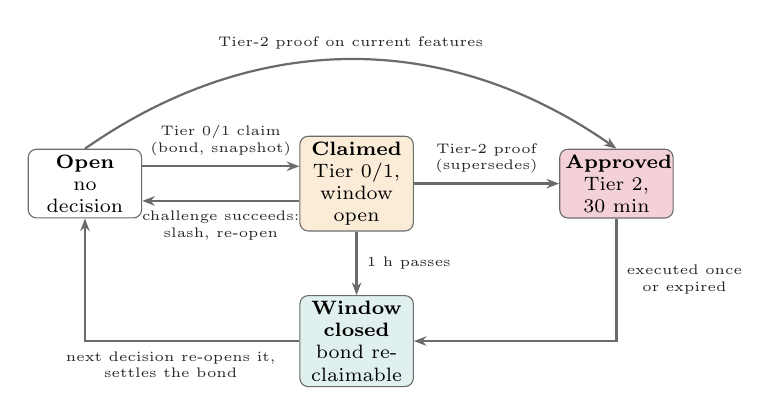
\begin{tikzpicture}[
      font=\scriptsize,
      st/.style={draw=muted,rounded corners=3pt,align=center,inner sep=2pt,minimum height=0.85cm,text width=1.3cm},
      arr/.style={-{Stealth[length=1.6mm]},thick,draw=muted},
      lb/.style={font=\tiny,align=center,text=black!85}]
    \node[st] (open) at (0,0) {\textbf{Open}\\no decision};
    \node[st,fill=tierone!20] (claim) at (3.45,0) {\textbf{Claimed}\\Tier 0/1,\\window open};
    \node[st,fill=tiertwo!25] (final) at (6.75,0) {\textbf{Approved}\\Tier 2, 30 min};
    \node[st,fill=tierzero!15] (closed) at (3.45,-2.0) {\textbf{Window closed}\\bond reclaimable};
    \draw[arr] ([yshift=2.2mm]open.east) -- node[above,lb]{Tier 0/1 claim\\(bond, snapshot)} ([yshift=2.2mm]claim.west);
    \draw[arr] ([yshift=-2.2mm]claim.west) -- node[below,lb]{challenge succeeds:\\slash, re-open} ([yshift=-2.2mm]open.east);
    \draw[arr] (claim) -- node[above,lb]{Tier-2 proof\\(supersedes)} (final);
    \draw[arr] (open.north) to[out=35,in=145] node[above,lb]{Tier-2 proof on current features} (final.north);
    \draw[arr] (claim) -- node[right,lb]{1 h passes} (closed);
    \draw[arr] (closed.west) -| node[below,lb,pos=0.3]{next decision re-opens it,\\settles the bond} (open.south);
    \draw[arr] (final.south) |- node[right,lb,pos=0.25]{executed once\\or expired} (closed.east);
  \end{tikzpicture}
  \caption{Position lifecycle. Cheap claims block only other cheap claims for one window; a Tier-2 proof of current high risk always proceeds and approves one liquidation, executed by the liquidator within 30 minutes or expired.}
  \label{fig:lifecycle}
\end{figure}

\subsection{Incentives}
\label{sec:design-incentives}

An optimistic tier is secure only if someone checks it. A watcher slashes a false claim only when the bond it wins exceeds the challenge's cost, about 0.68\,M gas: with a fixed 0.01\,ETH bond that stops being true above 14.7\,gwei (Section~\ref{sec:eval-incentives}), so at ordinary L1 gas prices nobody has a reason to watch, the verifier's dilemma. TrustTier closes the gap in four ways.
\begin{itemize}
  \item \textbf{Gas-scaled bonds.} A claim must post $\max(0.01\,\mathrm{ETH},\ 1.5\,\mathrm{M}\cdot\mathrm{basefee})$, read from \code{block.basefee} at the claim. The bond covers a challenge at any gas price and stays profitable while the base fee at challenge time is below 2.2$\times$ the base fee at the claim.
  \item \textbf{Rewards for honest work.} The lending protocol funds a reward pool; an unchallenged claim earns \code{claimReward} when its bond is settled, at most once per position per day, so attesting to safe positions is paid work and cannot be farmed by re-claiming.
  \item \textbf{Commit-reveal challenges.} A challenger first commits $\mathrm{keccak256}(\mathrm{challenger}, \mathrm{position}, \mathrm{snap}, \mathrm{keccak256}(\mathrm{proof}))$ and reveals the proof at least one block later. Once any commit exists for a claim, the one-step \code{challengeDecision} is closed for it, so a bot that copies a revealed proof from the mempool has no commit and cannot claim the bond.
  \item \textbf{Must-open commitments} (Section~\ref{sec:design-challenge}) make a Tier-1 claim self-checking.
\end{itemize}

\subsection{Executing decisions}
\label{sec:design-consumer}

A decision nobody acts on is only a record. \code{TrustTierLiquidator} is the lending protocol's one path to liquidation: \code{liquidate(position)} calls \code{consumeApproval}, which only the configured liquidator may call and which succeeds only on an open, unexpired Tier-2 approval, then asks the protocol to execute. The demo pool performs a \emph{soft} liquidation: it closes 50\% of the debt and moves collateral worth the repaid debt plus a 5\% bonus to whoever called, which pays the keeper for the proof. One proof buys exactly one liquidation. Because the model is proven on-chain, the pool may act \emph{before} LTV reaches the threshold, which is the reason to use a model at all; the protocol's own health-factor liquidation stays in force as a fallback.

\paragraph{Slow proofs.} A Tier-2 proof takes about 16\,s, longer than a block, and a feed update in between changes $q$ and invalidates it. Anyone may \code{anchorFeatures(position)}, which stores the hash of the current $q$ and $\delta$. For 10 minutes a proof on the anchored features is accepted, but only while the position has not become safer than at the anchor ($\delta_\mathrm{now}\le\delta_\mathrm{anchor}$). The router anchors only when a feed moved during proving, and then proves once more.

\subsection{Governance and model registry}

\code{ModelRegistry} holds the set of trusted model hashes; a revoked hash cannot be revoked again or silently re-registered. \code{setTier2Verifier(verifier, modelHash)} binds the verifier to the one model it encodes, and Tier-2 decisions must cite exactly that hash. All owner functions (registering or revoking models, swapping the verifier, changing the position source or feed staleness limits) belong to an OpenZeppelin \code{TimelockController}~\cite{ozTimelock}, whose only proposer and executor is an M-of-N multisig. Every change therefore needs M signatures and a public delay (goal G7).

\subsection{Designing for concurrent execution}
\label{sec:design-concurrency}

Parallel execution engines gain only when transactions touch disjoint state~\cite{gelashvili2023blockstm,saraph2020empirical}. TrustTier follows one rule: every storage write is keyed by a single position, account or model. The midterm audit log broke it by appending every decision to one array, whose length slot every transaction wrote; \code{TierAuditLog} now stores one record per position and history is read from events. Per-position engine state is packed into three slots (claimant and bond; deadline and three flags; snapshot), which also saves about 46\,k gas per cheap claim.

Opcode traces of whole blocks (Section~\ref{sec:eval-traces}) exposed one more shared write that storage keys do not show: a bond paid as \code{msg.value} changes the engine's ETH balance. On an engine that treats a balance change as a read-modify-write, every cheap claim in a block then conflicts with every other. We therefore added \emph{deposit-funded bonds}: \code{deposit()} pre-funds the claimant's own balance in \code{pendingWithdrawals}, a claim sent without ETH draws \code{MIN\_BOND} from it, and reclaimed or slashed bonds are recycled the same way. Such a claim touches only its claimant's slot, for 5,238 extra gas. Rewards are paid when a bond is settled, not when a claim is made, so the reward pool's shared balance is never written by a claim.

\subsection{Why a SNARK, not a STARK}
\label{sec:design-stark}

zk-STARKs need no trusted setup and resist quantum attacks~\cite{bensasson2019stark}, so they are the natural alternative for Tier~2. The right choice depends on how proofs are used, and TrustTier verifies proofs one at a time, inside the liquidation that depends on them. Published measurements favour a SNARK for that pattern (Table~\ref{tab:stark}). For the same statement, a STARK proof was 68,564 bytes against 384 bytes for Groth16, about 178 times larger~\cite{nainwal2025comparative}. Verifying one StarkWare proof on Ethereum costs about 9\,M gas, affordable only because one proof covers a whole batch~\cite{epicweb3packing}. A Cairo proof of a tiny Fibonacci program is 166\,KB~\cite{zksecurityadapter}. Even STARK-based production systems wrap their STARK in a Groth16 proof for the on-chain step~\cite{risczerorecursion}. Our Halo2 proof is 3,584 bytes and verifies for 621,921 gas. It is larger than a Groth16 proof because Halo2/KZG uses a universal, circuit-independent setup, and EZKL turns an ONNX model into a circuit and verifier directly~\cite{ezkl}. We accept a trusted setup and no post-quantum security; if Tier-2 decisions were batched into a periodic settlement proof, a STARK's economics would win.

\begin{table}[t]
  \caption{SNARK vs STARK for Tier~2. TrustTier numbers are measured; STARK numbers are from the cited sources.}
  \label{tab:stark}
  \footnotesize
  \setlength{\tabcolsep}{3pt}
  \begin{tabularx}{\columnwidth}{@{}lLL@{}}
    \toprule
    \textbf{Criterion} & \textbf{Halo2/KZG (TrustTier)} & \textbf{STARK} \\
    \midrule
    Proof size & 3,584 B & 68,564 B vs 384 B Groth16~\cite{nainwal2025comparative}; 166\,KB Cairo~\cite{zksecurityadapter} \\
    On-chain verification & 621,921 gas & $\approx$9\,M gas, amortized over a batch~\cite{epicweb3packing} \\
    ML tooling & EZKL: ONNX $\to$ circuit $\to$ verifier & Less mature for small ONNX models \\
    Trusted setup & Required (KZG SRS) & None \\
    Post-quantum & No & Yes \\
    Fits & One proof per decision & Batched settlement \\
    \bottomrule
  \end{tabularx}
\end{table}

%% ===================================================================
\section{Implementation}
\label{sec:impl}

Figure~\ref{fig:arch} shows the system.

\begin{figure*}[t]
  \centering
  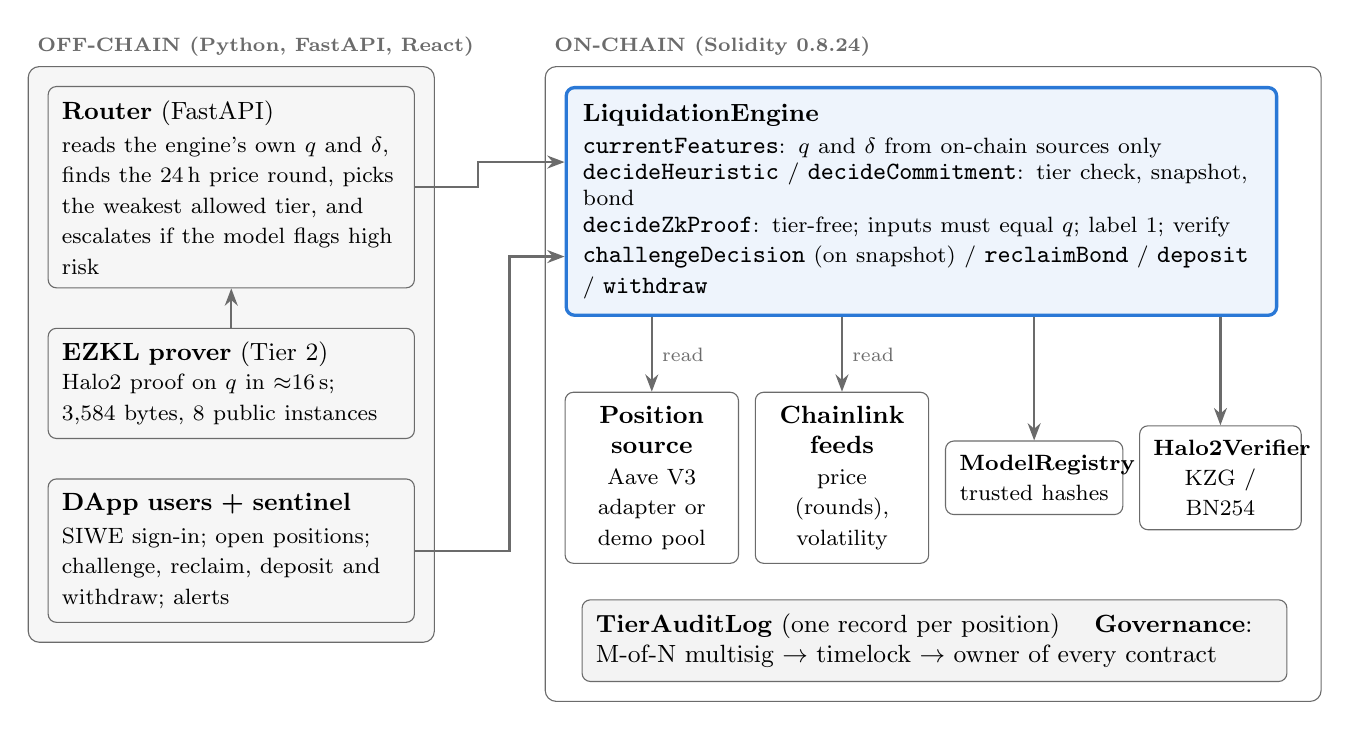
\begin{tikzpicture}[
      font=\small,
      box/.style={draw=muted,rounded corners=3pt,align=left,inner sep=5pt,text width=#1},
      box/.default=4.3cm,
      main/.style={draw=accent,very thick,fill=accent!8,rounded corners=3pt,align=left,inner sep=6pt,text width=8.6cm},
      arr/.style={-{Stealth[length=2.2mm]},thick,draw=muted},
      lbl/.style={font=\scriptsize,text=muted}]
    \node[box] (router) {\textbf{Router} (FastAPI)\\[1pt]\footnotesize reads the engine's own $q$ and $\delta$, finds the 24\,h price round, picks the weakest allowed tier, and escalates if the model flags high risk};
    \node[box,below=0.5cm of router] (prover) {\textbf{EZKL prover} (Tier 2)\\[1pt]\footnotesize Halo2 proof on $q$ in $\approx$16\,s;\\ 3,584 bytes, 8 public instances};
    \node[box,below=0.5cm of prover] (dapp) {\textbf{DApp users + sentinel}\\[1pt]\footnotesize SIWE sign-in; open positions; challenge, reclaim, deposit and withdraw; alerts};
    \node[main,right=1.9cm of router.north east,anchor=north west] (engine) {\textbf{LiquidationEngine}\\[2pt]\footnotesize
      \code{currentFeatures}: $q$ and $\delta$ from on-chain sources only\\
      \code{decideHeuristic} / \code{decideCommitment}: tier check, snapshot, bond\\
      \code{decideZkProof}: tier-free; inputs must equal $q$; label 1; verify\\
      \code{challengeDecision} (on snapshot) / \code{reclaimBond} / \code{deposit} / \code{withdraw}};
    \node[box=1.85cm,align=center,below=0.95cm of engine.south west,anchor=north west] (src) {\textbf{Position source}\\\footnotesize Aave~V3 adapter or demo pool};
    \node[box=1.85cm,align=center,right=0.2cm of src] (feeds) {\textbf{Chainlink feeds}\\\footnotesize price (rounds), volatility};
    \node[box=1.9cm,align=center,right=0.2cm of feeds] (reg) {\footnotesize\textbf{ModelRegistry}\\ trusted hashes};
    \node[box=1.7cm,align=center,right=0.2cm of reg] (ver) {\footnotesize\textbf{Halo2Verifier}\\ KZG / BN254};
    \node[draw=muted,fill=muted!8,rounded corners=3pt,align=left,inner sep=5pt,text width=8.6cm,below=0.45cm of feeds.south west,anchor=north west,xshift=-2.2cm] (gov) {\textbf{TierAuditLog} (one record per position) \quad \textbf{Governance}: M-of-N multisig $\to$ timelock $\to$ owner of every contract};
    \begin{scope}[on background layer]
      \node[draw=muted,fill=muted!6,rounded corners=4pt,inner sep=7pt,fit=(router)(dapp),label={[lbl,anchor=south west,font=\scriptsize\bfseries]north west:OFF-CHAIN (Python, FastAPI, React)}] {};
      \node[draw=muted,rounded corners=4pt,inner sep=7pt,fit=(engine)(src)(ver)(gov),label={[lbl,anchor=south west,font=\scriptsize\bfseries]north west:ON-CHAIN (Solidity 0.8.24)}] {};
    \end{scope}
    \draw[arr] (prover) -- (router);
    \draw[arr] (router.east) -- ++(0.8,0) |- ([yshift=5mm]engine.west);
    \draw[arr] (dapp.east) -- ++(1.2,0) |- ([yshift=-7mm]engine.west);
    \draw[arr] (src.north |- engine.south) -- node[right,lbl]{read} (src.north);
    \draw[arr] (feeds.north |- engine.south) -- node[right,lbl]{read} (feeds.north);
    \draw[arr] (reg.north |- engine.south) -- (reg.north);
    \draw[arr] (ver.north |- engine.south) -- (ver.north);
  \end{tikzpicture}
  \caption{TrustTier architecture. The engine reads every input itself; the router only chooses a tier the engine will accept and supplies proofs. Users act from their own wallets.}
  \label{fig:arch}
\end{figure*}

\paragraph{Contracts.} \code{LiquidationEngine} (14,100 bytes deployed), \code{TrustTierLiquidator}, \code{ModelRegistry}, \code{TierAuditLog}, the EZKL-generated \code{Halo2Verifier} (15,612 bytes, under the 24,576-byte EIP-170 limit~\cite{eip170}), \code{AaveV3PositionSource}, \code{MockLendingPool}, \code{TrustTierMultisig} and \code{TrustTierTimelock}, in Solidity 0.8.24 with OpenZeppelin~5. Every revert is a custom error. EZKL's verifier reverts on a bad proof instead of returning false, so the engine wraps it in \code{try/catch}. The Aave adapter cannot read account age or top-up times from Aave, which stores neither; it records registration time and lets anyone \code{poke} an account to record a top-up when its aToken's \emph{scaled} balance (deposits without accrued interest) grows. Both are derived from on-chain state only.

\paragraph{Risk model.} A 5$\to$8$\to$1 multilayer perceptron (scikit-learn) on the five normalized features, exported to ONNX with logits clipped to $\pm8$ inside the graph. Synthetic labels are centred near LTV~0.75, just below a 0.80 threshold. Validation accuracy is 95.9\% and ROC-AUC 0.995. The model's keccak256 hash is what \code{ModelRegistry} stores.

\paragraph{Circuit.} EZKL~23.0.5 with input and parameter scale $2^{10}$, public inputs, private parameters and public outputs, $2^{16}$ rows, and one inner column (\code{num\_inner\_cols=1}), which keeps the verifier under the EIP-170 limit; a Poseidon-hashed input variant did not fit. EZKL's witness generation hangs on inputs outside its calibrated range, so we calibrate over the whole normalized domain including all corners, and check circuit/ONNX label agreement on 200 random feature vectors (0 disagreements). The 8.4\,MB SRS is self-generated; EZKL's setup is deterministic for a given SRS, so the 575\,MB proving key is not shipped and is rebuilt in 12\,s, with a check that it matches the shipped verification key and verifier.

\paragraph{Router, sentinel and DApp.} The FastAPI router reads the engine's own view of a position, picks the weakest tier the chain accepts, runs the model, and escalates a Tier-1 position to Tier~2 when the model flags it, since a cheap ``safe'' claim on it would be false and slashable. A watcher endpoint builds a Tier-2 proof on a claim's snapshot (read from \code{FeaturesSnapshotted}). The React DApp signs users in with Sign-In with Ethereum (ERC-4361~\cite{eip4361}); users open demo positions, see the contract's features, $\delta$, allowed tier and the model's verdict, push mock prices, run a five-step guided demo, watch open claims and pending approvals with live countdowns, and challenge (commit, then reveal), settle bonds, execute liquidations and withdraw from their own wallets. When no router is reachable, for example on the hosted site, it runs the contract's rules, the real model (exported weights, checked against ONNX) and the measured gas in the browser, clearly labelled as a simulation. The sentinel polls events and raises a critical alert when a challenge succeeds. There is no database: on-chain events are the history.

\paragraph{Testing.} 126 Hardhat tests cover every function and custom error, real proofs against the real verifier end to end, the Aave adapter, governance, tier enforcement, snapshots, lifecycle, deposits, gas-scaled bonds, rewards, reveals, commit-reveal challenges, anchors, the liquidator, the sequencer check and a Chainlink phase boundary. 82 Python tests cover the feature mirror against real proof instances, the tier rule, commitments, the 24-hour round search (against brute force on 50 random histories), the cost model, the parallel-execution simulator and the DApp's exported model.

%% ===================================================================
\section{Evaluation}
\label{sec:eval}

\subsection{Setup}

All measurements ran on one 2-vCPU Intel Xeon (2.8\,GHz) machine with 7\,GB of RAM: Hardhat~2.29 (in-process chain or local node), Node~22, Python~3.13, EZKL~23.0.5, scikit-learn~1.9, ONNX Runtime~1.29. Gas is measured by executing every entry point on a fresh chain (\code{scripts/measure\_gas.js}), with the real verifier and real proofs, and includes the 21,000-gas transaction base. The evaluation set has 374 positions: 74 snapshots of one real Aave~V2 wallet's health-factor history, including a genuine liquidation, with each snapshot's own threshold; and 300 synthetic positions spread across safe, watch and critical LTV bands with a 0.80 threshold. Cost results apply the measured per-tier gas to this set; re-proving hundreds of positions would change nothing, because proving time and verification gas depend on the fixed circuit, not on the input.

\subsection{Proving and verification}

Table~\ref{tab:proving} summarizes the Tier-2 pipeline. Three sample positions are defined by on-chain parameters (a high-risk position at LTV~0.93, a low-risk one at 0.20, and a watch-band position at 0.72 that the model flags) and proved for real. The contract's computed $q$ equals each proof's first five instances.

\begin{table}[t]
  \caption{Tier-2 proving pipeline (measured).}
  \label{tab:proving}
  \footnotesize
  \begin{tabularx}{\columnwidth}{@{}Lr@{}}
    \toprule
    Circuit rows / input scale & $2^{16}$ / $2^{10}$ \\
    Public instances & 8 (5 features, label, 2 probabilities) \\
    Proving time (3 samples; 4 router runs) & 16.0--16.5\,s; 15.5--16.2\,s \\
    Proving key / verification key / SRS & 575\,MB / 141\,KB / 8.4\,MB \\
    Proving-key rebuild from SRS & 12.1\,s \\
    Proof calldata & 3,584 bytes \\
    Verifier: deployed size / deployment gas & 15,612 B / 3,422,602 \\
    \code{verifyProof} alone / full \code{decideZkProof} & 621,921 / 878,059 gas \\
    Circuit vs ONNX label agreement & 200 / 200 \\
    \bottomrule
  \end{tabularx}
\end{table}

\subsection{Gas of every entry point}

Table~\ref{tab:gas} lists every entry point. \code{currentFeatures}, called as a view, costs 92,510 gas including the base cost. It is the price of verified inputs and is included in every \code{decide*} row. A challenge with a real proof costs 678,771 gas, below a full Tier-2 decision because it checks a stored snapshot instead of recomputing features; committing first adds 94,771. Executing an approval costs 96,402 gas.

\begin{table}[t]
  \caption{Measured gas per transaction (real verifier and real proofs for Tier~2 and challenge).}
  \label{tab:gas}
  \footnotesize
  \begin{tabularx}{\columnwidth}{@{}Lr@{}}
    \toprule
    \code{decideHeuristic} (bond as \code{msg.value} / from deposit) & 269,534 / 274,772 \\
    \code{decideCommitment} (\code{msg.value} / deposit) & 340,072 / 345,310 \\
    \code{revealCommitment} & 39,089 \\
    \code{decideZkProof} (current / anchored features) & 878,059 / 882,059 \\
    \code{anchorFeatures} & 140,461 \\
    \code{challengeDecision} / \code{commitChallenge} + \code{revealChallenge} & 678,771 / 94,771 + 678,838 \\
    \code{liquidate} (soft liquidation through the liquidator) & 96,402 \\
    \code{reclaimBond} / \code{withdraw} / \code{deposit} & 55,980 / 30,004 / 45,025 \\
    \code{currentFeatures} (view) & 92,510 \\
    \code{registerModel} / \code{revokeModel} / \code{setTier2Verifier} & 139,257 / 28,150 / 30,496 \\
    Losing racer (\code{PositionAlreadyFinalized}, live node) & 26,149 \\
    Deploy: engine / verifier / demo pool / liquidator & 3,286,971 / 3,422,602 / 847,742 / 201,232 \\
    \bottomrule
  \end{tabularx}
\end{table}

\subsection{Cost of tiering}

Table~\ref{tab:cost} applies the measured gas to the evaluation set, charging every Tier-1 claim its mandatory reveal. Tiering spends 210.3\,M gas where proving every position would spend 328.4\,M, a 36.0\% saving, and needs 165 proofs instead of 374, which cuts off-chain proving from 6,096\,s to 2,690\,s. The figure is conservative: the 9 Tier-2 positions whose proof shows low risk submit no transaction but are charged full gas. Always using Tier~0 would cost 100.8\,M gas but verify nothing.

\begin{table}[t]
  \caption{Gas of TrustTier vs always proving (M = million gas).}
  \label{tab:cost}
  \footnotesize
  \setlength{\tabcolsep}{3.5pt}
  \begin{tabular}{@{}lrcrrr@{}}
    \toprule
    \textbf{Dataset} & \textbf{N} & \textbf{T0/T1/T2} & \textbf{Tiered} & \textbf{All-zk} & \textbf{Saving} \\
    \midrule
    Real Aave V2 & 74 & 26/7/41 & 45.7\,M & 65.0\,M & 29.7\% \\
    Synthetic & 300 & 100/76/124 & 164.6\,M & 263.4\,M & 37.5\% \\
    \midrule
    \textbf{Combined} & \textbf{374} & \textbf{126/83/165} & \textbf{210.3\,M} & \textbf{328.4\,M} & \textbf{36.0\%} \\
    \bottomrule
  \end{tabular}
\end{table}

\subsection{Ablations of the design}
\label{sec:eval-ablation}

Table~\ref{tab:ablation} removes one component at a time on the same 374 positions.

\begin{table}[t]
  \caption{Ablations on the 374 positions (measured per-tier gas).}
  \label{tab:ablation}
  \footnotesize
  \setlength{\tabcolsep}{3pt}
  \begin{tabularx}{\columnwidth}{@{}P{2.7cm}rL@{}}
    \toprule
    \textbf{Variant} & \textbf{Saving} & \textbf{Cost of the change} \\
    \midrule
    TrustTier (deployed) & 36.0\% & -- \\
    No Tier-1 escalation & 39.1\% & 21 false, slashable cheap claims \\
    No Tier~1 (Tier~0 or Tier~2 only) & 23.3\% & Tier~1 is worth 12.7 points \\
    Tier-1 band $B_1=0$ & 37.3\% & 7 claims a 5\% drop breaches \\
    Always Tier~0 & 69.3\% & Nothing verified; 157 model-flagged positions unchecked \\
    \bottomrule
  \end{tabularx}
\end{table}

Escalation costs 3.1 points and buys honesty: without it, 21 cheap claims would contradict the router's own model (and, now that commitments must be opened, forfeit their bonds). Removing Tier~1 costs 12.7 points, which shows that the middle tier carries much of the saving. Section~\ref{sec:eval-bands} explains the band rows.

\paragraph{How the design evolved.} Table~\ref{tab:versions} follows the same measures through four versions. The midterm prototype was cheapest per decision because it checked almost nothing. Binding proofs to positions through an oracle-committed Poseidon hash fixed proof replay but added a 49,682-gas oracle transaction to every position and trusted the oracle. Verified inputs remove the oracle. Cheap tiers now pay for reading two feeds and storing a snapshot, while Tier~2 becomes cheaper: the proof has no in-circuit hash, and normalization shrank the circuit. The saving fell because the always-proving baseline also fell, but TrustTier's absolute cost is within 3.6\% of the midterm's (210.3\,M against 203.0\,M), now with input integrity, tier enforcement, proof binding, escalation, and the incentive layer, which adds about 3\,k gas per decision plus the Tier-1 reveal.

\begin{table}[t]
  \caption{Four versions of TrustTier on the same 374 positions.}
  \label{tab:versions}
  \scriptsize
  \setlength{\tabcolsep}{2pt}
  \begin{tabular}{@{}lrrrr@{}}
    \toprule
    & \textbf{Midterm} & \textbf{Oracle} & \textbf{Verified} & \textbf{Final} \\
    \midrule
    Tier 0 gas & 195,869 & 250,098 & 266,202 & 269,534 \\
    Tier 1 gas & 286,356 & 340,550 & 336,713 & 379,161 \\
    Tier 2 gas & 1,031,754 & 999,623 & 875,489 & 878,059 \\
    \code{verifyProof} gas & 849,607 & 741,069 & 621,921 & 621,921 \\
    Proof bytes & 5,696 & 4,480 & 3,584 & 3,584 \\
    Proving & 25\,s & 20\,s & 16\,s & 16\,s \\
    Tiers (T0/T1/T2) & 126/104/144 & 126/83/165 & 126/83/165 & 126/83/165 \\
    Saving & 47.4\% & 39.9\% & 37.1\% & 36.0\% \\
    Inputs from & router & oracle & contract & contract \\
    Tier enforced by & nobody & nobody & contract & contract \\
    Slashing pays at & any & $\le$15\,gwei & $\le$15\,gwei & any \\
    Liquidation executed & no & no & no & once, $\le$30\,min \\
    \bottomrule
  \end{tabular}
\end{table}

\subsection{Choosing the tier bands}
\label{sec:eval-bands}

The bands $B_0=0.15$ and $B_1=0.05$ are the two numbers TrustTier's guarantees hang on, so we asked how much the results depend on them. Replaying the 374 positions over 34 band settings (Figure~\ref{fig:band-sensitivity}) shows that both can be argued for rather than assumed.

The Tier-1 band is a safety margin. A cheap claim is honest only while the position stays below its threshold for the one-hour window, and a claim made at $\delta > B_1$ survives a sudden collateral price drop $s$ whenever $B_1 \ge \theta s$. For $\theta=0.80$ and a severe 5\% hourly drop this requires $B_1 \ge 0.04$. The replay agrees: with $B_1=0$, seven cheap claims would be pushed past their threshold by such a drop; with $B_1=0.02$, three; with $B_1=0.05$, none.

The Tier-0 band trades gas for model oversight. With $B_1=0.05$, widening it from 0.08 to 0.30 lowers the saving from 38.7\% to 33.9\%, while the Tier-0 claims the model would flag fall from 5 to 2 at $B_0=0.10$, 1 at 0.15 and none from 0.20 (22 at $B_0=0.05$). Most of the safety is bought by 0.10; beyond it each step costs gas for little gain. The deployed $(0.15, 0.05)$ lies on the Pareto front of the grid over saving, flagged claims and exposed claims: no setting is better on all three. $B_0=0.10$ is an equally defensible choice that saves 1.6 more points for one more flagged claim.

The 0.80 threshold used for the synthetic stream matters less than it might appear. The contract never assumes it, and the real positions keep their own thresholds. Moving the synthetic threshold from 0.70 to 0.85 (Table~\ref{tab:threshold-sensitivity}) changes the saving from 23.9\% to 38.1\%, because the synthetic positions sit closer to or further from their boundary. The safety measures do not change: one flagged Tier-0 claim and no exposed claims at every threshold. Two caveats apply: ``flagged'' is the model's own verdict, not ground truth, and the 5\% drop is a stress assumption, not a measured bound.

% Generated by off-chain/evaluation/band_sensitivity.py - do not edit by hand.
% Needs pgfplots, booktabs and the paper's tierzero/tierone/tiertwo/accent/muted colors.
\begin{figure}[t]
\centering
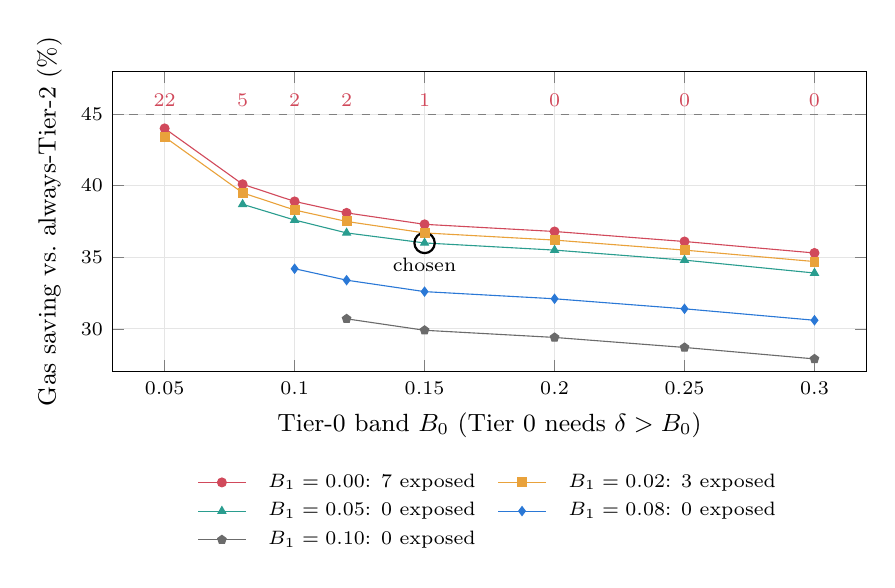
\begin{tikzpicture}
\begin{axis}[
  width=0.92\columnwidth, height=5.4cm,
  xlabel={Tier-0 band $B_0$ (Tier~0 needs $\delta > B_0$)},
  ylabel={Gas saving vs.\ always-Tier-2 (\%)},
  ymin=27, ymax=48, xmin=0.03, xmax=0.32,
  xtick={0.05,0.10,0.15,0.20,0.25,0.30},
  xticklabel style={/pgf/number format/fixed, /pgf/number format/precision=2},
  clip=false,
  legend columns=2,
  legend style={font=\scriptsize, at={(0.5,-0.30)}, anchor=north, draw=none, column sep=6pt},
  tick label style={font=\scriptsize}, label style={font=\small},
  grid=major, grid style={gray!20}]
\addplot[color=tiertwo, mark=*, mark size=1.6pt] coordinates {(0.05,44.0) (0.08,40.1) (0.1,38.9) (0.12,38.1) (0.15,37.3) (0.2,36.8) (0.25,36.1) (0.3,35.3)};
\addlegendentry{$B_1=0.00$: 7 exposed}
\addplot[color=tierone, mark=square*, mark size=1.6pt] coordinates {(0.05,43.4) (0.08,39.5) (0.1,38.3) (0.12,37.5) (0.15,36.7) (0.2,36.2) (0.25,35.5) (0.3,34.7)};
\addlegendentry{$B_1=0.02$: 3 exposed}
\addplot[color=tierzero, mark=triangle*, mark size=1.6pt] coordinates {(0.08,38.7) (0.1,37.6) (0.12,36.7) (0.15,36.0) (0.2,35.5) (0.25,34.8) (0.3,33.9)};
\addlegendentry{$B_1=0.05$: 0 exposed}
\addplot[color=accent, mark=diamond*, mark size=1.6pt] coordinates {(0.1,34.2) (0.12,33.4) (0.15,32.6) (0.2,32.1) (0.25,31.4) (0.3,30.6)};
\addlegendentry{$B_1=0.08$: 0 exposed}
\addplot[color=muted, mark=pentagon*, mark size=1.6pt] coordinates {(0.12,30.7) (0.15,29.9) (0.2,29.4) (0.25,28.7) (0.3,27.9)};
\addlegendentry{$B_1=0.10$: 0 exposed}
\node[font=\scriptsize, text=tiertwo] at (axis cs:0.05,46) {22};
\node[font=\scriptsize, text=tiertwo] at (axis cs:0.08,46) {5};
\node[font=\scriptsize, text=tiertwo] at (axis cs:0.1,46) {2};
\node[font=\scriptsize, text=tiertwo] at (axis cs:0.12,46) {2};
\node[font=\scriptsize, text=tiertwo] at (axis cs:0.15,46) {1};
\node[font=\scriptsize, text=tiertwo] at (axis cs:0.2,46) {0};
\node[font=\scriptsize, text=tiertwo] at (axis cs:0.25,46) {0};
\node[font=\scriptsize, text=tiertwo] at (axis cs:0.3,46) {0};
\draw[dashed, gray] (axis cs:0.03,45) -- (axis cs:0.32,45);
\node[draw, circle, inner sep=2.6pt, thick] at (axis cs:0.15,36.0) {};
\node[font=\scriptsize, anchor=north] at (axis cs:0.15,35.6) {chosen};
\end{axis}
\end{tikzpicture}
\caption{Gas saving over 374 positions as the tier bands vary. Red numbers along the top: Tier-0
claims the model would flag high risk at each $B_0$ (independent of $B_1$). ``Exposed'': cheap
claims that a sudden 5\% collateral price drop would push past the liquidation threshold. The
circled point is the deployed setting ($B_0=0.15$, $B_1=0.05$).}
\label{fig:band-sensitivity}
\end{figure}

\begin{table}[t]
\centering\small
\caption{Sensitivity to the synthetic stream's liquidation threshold (bands fixed at 0.15/0.05; real positions keep their own thresholds).}
\label{tab:threshold-sensitivity}
\begin{tabular}{lcccc}
\toprule
Threshold & Tiers 0/1/2 & Saving & Tier-0 flagged & Exposed \\
\midrule
0.70 & 110/23/241 & 23.9\% & 1 & 0 \\
0.75 & 126/44/204 & 30.0\% & 1 & 0 \\
0.80 & 126/83/165 & 36.0\% & 1 & 0 \\
0.85 & 163/52/159 & 38.1\% & 1 & 0 \\
\bottomrule
\end{tabular}
\end{table}


\subsection{Model calibration and fidelity}

The midterm model was trained on labels centred at LTV~0.5, below almost every position, so it flagged 84.1\% of Tier-0 positions as high risk and made the Tier-0 check meaningless. Model~v2 centres labels near the threshold and trains on normalized features: it flags 1 of 126 Tier-0 positions (0.8\%), its validation accuracy is 95.9\% (ROC-AUC 0.995), and the circuit agrees with the ONNX model on all 200 random inputs, so the proven label is the model's label. Of the 165 Tier-2 positions, 9 are scored low risk; their proof shows label~0, the engine would reject the liquidation, and the router submits nothing. Proximity to the boundary alone never liquidates a position; the proven model output does.

\subsection{Against the health-factor rule}
\label{sec:eval-hf}

Is a model worth its gas compared with the rule every protocol already has? \code{evaluation/hf\_baseline.py} simulates 3,000 positions (initial LTV 0.40--0.79, $\theta=0.80$) for 30 days on identical price paths: a daily random walk with each position's own 30-day volatility, a common market factor (correlation 0.6) and a 2\% daily chance of a market-wide crash of 12--30\%. Debt is constant and borrowers never top up, a stress test rather than a forecast. Three policies act on the same paths. The \emph{health-factor rule} liquidates 50\% of the debt with a 5\% bonus once LTV $\ge\theta$. \emph{TrustTier} decides every position daily with its tiers and soft-liquidates (same close factor and bonus) when a proven model says high risk, with the health-factor rule as fallback. \emph{Always zk} proves every position daily. The model runs through the same ONNX file the circuit is compiled from, on the contract's quantized features.

\begin{table}[t]
  \caption{30-day stress test, 3,000 positions, identical price paths (seed 7). Bad debt and bonus as \% of initial debt; gas is decision gas per position-day.}
  \label{tab:hf}
  \footnotesize
  \setlength{\tabcolsep}{2.5pt}
  \begin{tabular}{@{}lrrrrrr@{}}
    \toprule
    \textbf{Policy} & \textbf{Forced} & \textbf{Insolv.} & \textbf{Bad debt} & \textbf{Bonus} & \textbf{Soft (unnec.)} & \textbf{Gas/day} \\
    \midrule
    HF rule & 2,461 & 61 & 0.018\% & 1.35\% & 0 & 0 \\
    TrustTier & 297 & 2 & 0.001\% & 1.67\% & 2,365 (323) & 322\,k \\
    Always zk & 297 & 2 & 0.001\% & 1.67\% & 2,368 (323) & 880\,k \\
    \bottomrule
  \end{tabular}
\end{table}

Table~\ref{tab:hf} shows the trade. Acting on the proven model cuts forced liquidations at the boundary by 88\% and insolvencies from 61 to 2; over ten further scenarios the mean bad debt falls from 0.087\% to 0.022\% of debt and insolvencies from 198 to 45. The costs are real. Borrowers pay more liquidation bonus in total (1.67\% against 1.35\% of debt), because soft liquidations are more frequent though smaller, and 323 of the 1,264 soft-liquidated positions (26\%) would never have reached the threshold. TrustTier gives the same protection as proving everything for 63\% less decision gas, because its tiers prove only near the boundary.

\subsection{Incentives and where TrustTier pays}
\label{sec:eval-incentives}

\code{evaluation/bond\_economics.py} prices the challenge game with measured gas. With the original fixed 0.01\,ETH bond, slashing a false claim loses money above 14.7\,gwei (12.9\,gwei with commit-reveal): the verifier's dilemma at ordinary L1 prices. The gas-scaled bond pays a watcher at every gas price, for example $+0.016$\,ETH at 20\,gwei and $+0.16$\,ETH at 200\,gwei, and stays profitable while the base fee at challenge time is under 1.94$\times$ the claim's.

Decision gas also decides where TrustTier is worth deploying (Table~\ref{tab:viability}). With one decision per position per day and a budget of 0.5\% of the debt per year, daily monitoring on L1 only pays for positions above \$353\,k (5\,gwei) to \$1.4\,M (20\,gwei). On a rollup at an effective 0.05\,gwei it pays from \$3.5\,k, ordinary retail size. TrustTier's natural home is therefore an L2 lending market, or L1 with a slower cadence for Tier-0 positions.

\begin{table}[t]
  \caption{Cost of daily decisions per position (ETH = \$3,000) and the smallest debt for which a year costs under 0.5\% of it.}
  \label{tab:viability}
  \footnotesize
  \setlength{\tabcolsep}{3pt}
  \begin{tabular}{@{}lrrrr@{}}
    \toprule
    & \multicolumn{2}{c}{\textbf{TrustTier}} & \multicolumn{2}{c}{\textbf{Always zk}} \\
    \textbf{Network} & \textbf{\$/yr} & \textbf{Min. debt} & \textbf{\$/yr} & \textbf{Min. debt} \\
    \midrule
    L1, 20\,gwei & 7,062 & 1.41\,M & 19,279 & 3.86\,M \\
    L1, 5\,gwei & 1,766 & 353\,k & 4,820 & 964\,k \\
    Rollup, 0.05\,gwei & 17.7 & 3.5\,k & 48.2 & 9.6\,k \\
    \bottomrule
  \end{tabular}
\end{table}

\subsection{Real outcomes}

The model's validation accuracy is measured on synthetic labels that are a formula of its own inputs, so it says little about real risk. \code{evaluation/outcome\_labels.py} instead labels real Aave~V2 snapshots by what happened: 1 if the health factor fell below 1 within 7 days. On the one wallet we hold (73 labelled snapshots, one positive) the deployed model reaches ROC-AUC 0.861 against 0.819 for a health-factor warning at 1.15, both with recall 1 and low precision. One wallet is a case study, not a statistic; the script runs unchanged on Cred Protocol's complete 35,524-wallet dataset and retrains a candidate model on outcome labels with a time-ordered split, which is the evaluation we would cite next.

\subsection{Concurrency}
\label{sec:eval-concurrency}

We study concurrency at three levels of realism: a modelled scheduler, as at the midterm; opcode-traced blocks executed by simulated parallel engines with 1 to 64 threads; and real competing liquidator threads on a live node.

\paragraph{Modelled scheduling.} Modelling each decision's read/write set and scheduling a batch greedily into conflict-free rounds, the array-based audit log needs one round per decision (374 rounds for 374 decisions), and per-position storage needs one round at every batch size from 50 to 2,000 and every tier mix from 80/15/5 to 10/20/70. Modelled same-position contention of 5--50\% raises this to 3--6 rounds.

\paragraph{Traced read/write sets.}
\label{sec:eval-traces}
Models can miss shared state, so we measured it. For each scenario, \code{scripts/concurrency\_trace.js} deploys the contracts with three markets, opens the positions, puts a whole batch of decisions from distinct liquidator accounts into \emph{one block}, mines it, and replays every transaction with \code{debug\_traceTransaction}. From the opcode trace we record every storage slot read (\code{SLOAD}) and written (\code{SSTORE}) in each contract, following the call stack, and every account balance moved. We then simulate three ways to execute the block, using each transaction's measured gas as its duration, with Tier~2 rescaled to the real-verifier cost: \emph{strict rounds} (any read/write overlap conflicts); a \emph{pre-computed schedule}, in which the block producer publishes a dependency graph that validators replay on $T$ threads~\cite{dickerson2017adding,anjana2019efficient}; and an \emph{optimistic} Block-STM-style engine~\cite{gelashvili2023blockstm}, in which $T$ threads execute speculatively in block order, only read-after-write dependencies count, and a transaction that read a value a lower transaction later wrote is aborted and re-executed. Fees to the block producer are deferred, as in every parallel EVM. Bond transfers into the engine are modelled two ways: as a commutative balance delta, or as a read-modify-write of the engine's balance. Table~\ref{tab:parallel} and Figures~\ref{fig:speedup}--\ref{fig:contention} report the results.

\begin{table*}[t]
  \caption{Parallel execution of traced blocks. ``Delta'': bond transfers are commutative balance deltas; ``RMW'': they read-modify-write the engine's ETH balance. Speedup = sequential gas / makespan for the pre-computed schedule (s) and the optimistic engine (o); Rounds: strict conflict-free rounds; Ab: aborts; Rev.: reverted.}
  \label{tab:parallel}
  \scriptsize
  \setlength{\tabcolsep}{2.6pt}
  \begin{tabular}{@{}llrrrrrrrl@{}}
    \toprule
    \textbf{Scenario (one block)} & \textbf{Bonds} & \textbf{Txs} & \textbf{Rev.} & \textbf{Rounds} & \textbf{16 thr s/o} & \textbf{64 thr s/o} & \textbf{Ab@16} & \textbf{Ab@64} & \textbf{Hottest shared write} \\
    \midrule
    Final design, 374 decisions & delta & 374 & 0 & 1 & 15.32 / 15.32 & 54.75 / 54.75 & 0 & 0 & none \\
    Final design, 374 decisions & RMW & 374 & 0 & 209 & 3.33 / 3.33 & 3.33 / 3.33 & 208 & 208 & engine balance (209 txs) \\
    Deposit-funded bonds, 374 & either & 374 & 0 & 1 & 15.34 / 15.34 & 54.97 / 54.97 & 0 & 0 & none \\
    Midterm array audit log, 374 & either & 374 & 0 & 374 & 1.00 / 1.00 & 1.00 / 1.00 & 373 & 373 & log length slot (374 txs) \\
    \midrule
    Final, 50 / 100 / 200 decisions & delta & -- & 0 & 1 & 13.2--15.0 & 31.4--48.4 & 0 & 0 & none \\
    Contention 5\% (200 + 10 dups) & delta & 210 & 10 & 2 & 15.00 / 15.00 & 48.55 / 49.44 & 0 & 4 & none \\
    Contention 20\% (200 + 40) & delta & 240 & 40 & 2 & 15.09 / 15.13 & 48.37 / 52.82 & 2 & 17 & none \\
    Contention 50\% (200 + 100) & delta & 300 & 100 & 2 & 14.57 / 15.15 & 42.78 / 49.35 & 11 & 49 & none \\
    Contention 20\% & RMW & 240 & 40 & 138 & 3.33 / 3.33 & 3.33 / 3.33 & 138 & 145 & engine balance \\
    1 / 3 / 6 oracle heartbeats & delta & 201--206 & 0 & 2--3 & 15.0 / 14.6--14.8 & 47.3--48.5 / 42.3--45.7 & 4--6 & 16--27 & price feeds \\
    Tier mix 80/15/5, 10/20/70 (s = o) & delta & 200 & 0 & 1 & 15.57, 15.12 & 43.58, 53.80 & 0 & 0 & none \\
    One liquidator sends all 200 & delta & 200 & 0 & 200 & 1.00 / 0.99 & 1.00 / 0.99 & 199 & 199 & sender nonce \\
    \bottomrule
  \end{tabular}
\end{table*}

\begin{figure}[t]
  \centering
  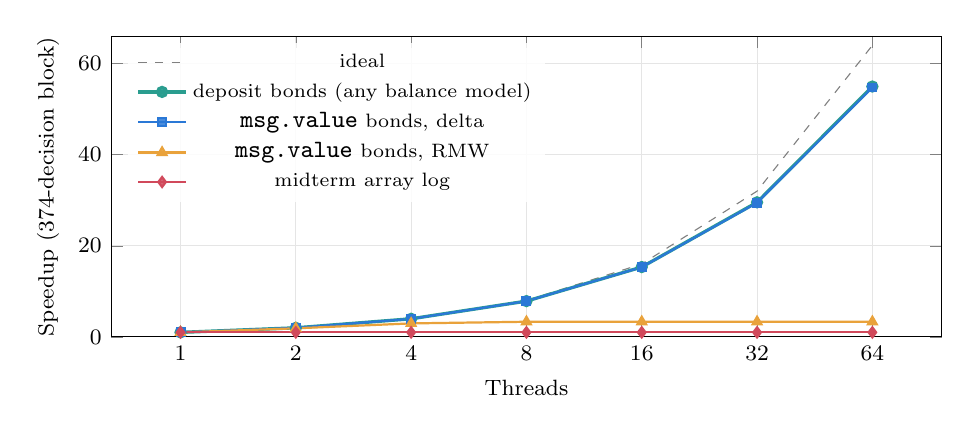
\begin{tikzpicture}
    \begin{axis}[
        width=\columnwidth, height=5.4cm,
        xmode=log, log basis x=2, xtick={1,2,4,8,16,32,64}, xticklabels={1,2,4,8,16,32,64},
        xlabel={Threads}, ylabel={Speedup (374-decision block)},
        ymin=0, ymax=66,
        label style={font=\footnotesize}, tick label style={font=\footnotesize},
        legend style={font=\scriptsize,at={(0.02,0.98)},anchor=north west,draw=none,fill=white,fill opacity=0.85,text opacity=1},
        grid=major, grid style={gray!20}]
      \addplot[gray,dashed] coordinates {(1,1) (2,2) (4,4) (8,8) (16,16) (32,32) (64,64)};
      \addlegendentry{ideal}
      \addplot[tierzero,very thick,mark=*,mark size=1.6pt] coordinates {(1,1) (2,2.0) (4,3.98) (8,7.86) (16,15.34) (32,29.55) (64,54.97)};
      \addlegendentry{deposit bonds (any balance model)}
      \addplot[accent,thick,mark=square*,mark size=1.4pt] coordinates {(1,1) (2,2.0) (4,3.97) (8,7.85) (16,15.32) (32,29.46) (64,54.75)};
      \addlegendentry{\code{msg.value} bonds, delta}
      \addplot[tierone,thick,mark=triangle*,mark size=1.8pt] coordinates {(1,1) (2,1.89) (4,2.97) (8,3.33) (16,3.33) (32,3.33) (64,3.33)};
      \addlegendentry{\code{msg.value} bonds, RMW}
      \addplot[tiertwo,thick,mark=diamond*,mark size=1.8pt] coordinates {(1,1) (2,1.0) (4,1.0) (8,1.0) (16,1.0) (32,1.0) (64,1.0)};
      \addlegendentry{midterm array log}
    \end{axis}
  \end{tikzpicture}
  \caption{Pre-computed-schedule speedup of one traced block of 374 decisions. Deposit-funded bonds keep the block parallel whichever way an engine treats balance updates.}
  \label{fig:speedup}
\end{figure}

\begin{figure}[t]
  \centering
  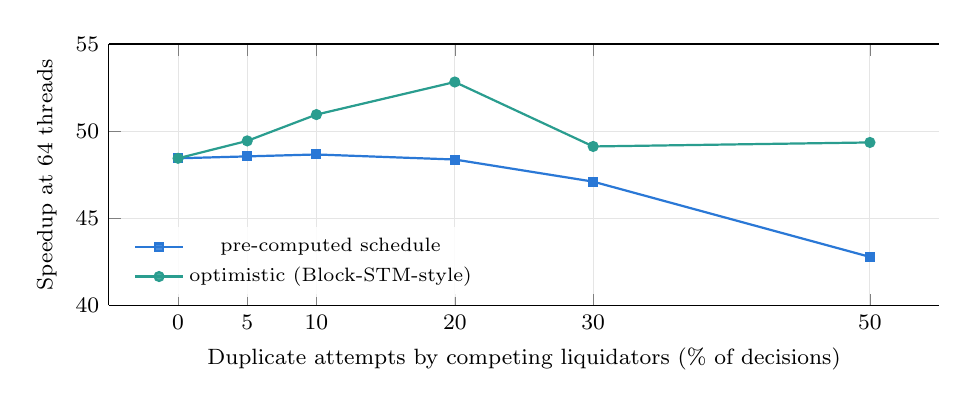
\begin{tikzpicture}
    \begin{axis}[
        width=\columnwidth, height=4.9cm,
        xlabel={Duplicate attempts by competing liquidators (\% of decisions)},
        ylabel={Speedup at 64 threads},
        xtick={0,5,10,20,30,50}, ymin=40, ymax=55,
        axis y line*=left,
        label style={font=\footnotesize}, tick label style={font=\footnotesize},
        legend style={font=\scriptsize,at={(0.02,0.03)},anchor=south west,draw=none,fill=white,fill opacity=0.85,text opacity=1},
        grid=major, grid style={gray!20}]
      \addplot[accent,thick,mark=square*,mark size=1.4pt] coordinates {(0,48.44) (5,48.55) (10,48.66) (20,48.37) (30,47.10) (50,42.78)};
      \addlegendentry{pre-computed schedule}
      \addplot[tierzero,thick,mark=*,mark size=1.6pt] coordinates {(0,48.44) (5,49.44) (10,50.95) (20,52.82) (30,49.12) (50,49.35)};
      \addlegendentry{optimistic (Block-STM-style)}

    \end{axis}
  \end{tikzpicture}
  \caption{Same-position contention in traced blocks of 200 decisions plus duplicates. Losing attempts revert at the lock and conflict only with the winner, so the block still needs just 2 strict rounds; speedup degrades gently. Optimistic aborts at 64 threads rise from 0 to 49 (Table~\ref{tab:parallel}).}
  \label{fig:contention}
\end{figure}

Five findings stand out.
\begin{enumerate}
  \item \textbf{Per-position storage parallelizes.} A block of 374 decisions has no shared storage write at all. It needs one strict round and reaches 15.3$\times$ on 16 threads and 54.8$\times$ on 64. Scaling falls short of ideal only because transaction durations differ: one Tier-2 decision costs 3.3 times a Tier-0 one, so the longest transactions bound the makespan. The midterm array log serializes the same block completely, whatever the engine.
  \item \textbf{The balance is the hidden hot spot.} Storage keys alone would suggest the final design is conflict-free. The traces show that every \code{msg.value} bond also writes the engine's ETH balance. Treated as a read-modify-write, that single location makes the 209 bonded claims a chain: 3.33$\times$ at any thread count, with 208 aborts in the optimistic engine. Deposit-funded bonds (Section~\ref{sec:design-concurrency}) restore 15.3$\times$ under both balance models, for 5,238 gas per claim. As on historical Ethereum, conflicts concentrate on a little popular state~\cite{saraph2020empirical}; tracing found ours where our model had not.
  \item \textbf{Racing liquidators cost little.} With 5--50\% duplicate attempts, losing attempts revert at the per-position lock, write nothing, and conflict only with the winner. The block still needs only 2 strict rounds, and 64-thread speedup stays at 42.8--52.8$\times$. Optimistic execution even beats the in-order schedule here: the schedule leaves a thread idle while it waits for a dependency, whereas the optimistic engine keeps every thread busy and pays only for a few aborts. The modelled scheduler had predicted 3--6 rounds, since it assumed losers write.
  \item \textbf{Oracle updates cause little conflict.} Chainlink heartbeat updates inside the block conflict with every later decision on that market, which reads the feed. Six updates raise strict rounds to 3 and cause 6 aborts at 16 threads, costing up to 2\% of optimistic speedup at 16 threads and 13\% at 64.
  \item \textbf{Parallelism needs many senders.} A single liquidator account submitting all 200 decisions serializes the block through its own nonce (1.0$\times$). Parallel execution helps a market of liquidators, not one bot.
\end{enumerate}

\paragraph{Competing liquidator threads on a live node.}
\label{sec:eval-race}
Finally, we ran $K$ liquidator bots as real concurrent threads, each with its own account and RPC connection, against a Hardhat node mining a block every second. Every bot tries to decide the same 30 positions (half Tier~0, half Tier~2) in its own random order and, like real racing bots, skips gas estimation, so losing transactions are mined and revert. Table~\ref{tab:race} shows that every position was decided exactly once at every $K$ (goal G6). Each losing attempt burns 26,149 gas, about a tenth of a Tier-0 decision, because the lock is checked before any external call; wasted gas grows linearly with the number of racers.

\begin{table}[t]
  \caption{$K$ competing liquidator threads on a live node (30 positions, 1-second blocks).}
  \label{tab:race}
  \footnotesize
  \setlength{\tabcolsep}{3pt}
  \begin{tabular}{@{}rrrrrcr@{}}
    \toprule
    \textbf{Bots} & \textbf{Tries} & \textbf{Won} & \textbf{Reverted} & \textbf{Wasted gas/pos.} & \textbf{Once} & \textbf{Blocks} \\
    \midrule
    1 & 30 & 30 & 0 & 0 & yes & 1 \\
    2 & 60 & 30 & 30 & 26,149 & yes & 1 \\
    4 & 120 & 30 & 90 & 78,447 & yes & 2 \\
    8 & 240 & 30 & 210 & 183,043 & yes & 3 \\
    16 & 480 & 30 & 450 & 392,235 & yes & 6 \\
    \bottomrule
  \end{tabular}
\end{table}

\paragraph{Limits of these results.} Ethereum clients execute blocks sequentially today. Our speedups are what a parallel engine could achieve on TrustTier's real access patterns, with gas as a stand-in for execution time, not measured wall-clock time of a parallel client.

\subsection{End-to-end validation}

With the real verifier on a local node, the router opened and routed streams across three markets, producing real Tier-2 decisions at about 878,000 gas and $\approx$16\,s of proving per position. Through the DApp, in a headless browser with an injected wallet, we opened a watch-band position (on-chain $\delta=800$\,bps, allowed tier~1, model: high risk), had the router claim Tier~1 dishonestly, generated a real proof on the claim's snapshot (16.2\,s), and challenged from a second wallet. The bond was credited to the challenger, the position re-opened, and the same proof then approved its liquidation at Tier~2. Claiming Tier~0 on that position reverted with \code{TierNotAllowed(\dots, 0, 800)}. With the final contracts, the DApp's five-step guided demo runs the same story on a local node and then executes the soft liquidation through \code{TrustTierLiquidator}, taking $\delta$ from 8.0\% to 22.1\%; a browser test drives it end to end, on-chain and in simulation mode.

%% ===================================================================
\section{Security Analysis}
\label{sec:security}

We reviewed the code STRIDE-style and with an independent review pass; Table~\ref{tab:security} condenses the 29 findings. We argue the goals of Section~\ref{sec:threat} as follows.

\textbf{G1 Input integrity:} every feature is computed by the contract from the position source and feeds within the transaction that uses it (finding~15). \textbf{G2 Tier soundness:} every cheap \code{decide*} recomputes $\delta$ and reverts below its band (finding~20). \textbf{G3 Proof binding:} \code{decideZkProof} compares the proof's five feature instances with its own computation and requires label~1, a registered model and the verifier's own model (findings 9--11). \textbf{G4 Accountability:} a challenge must prove high risk on the claim's snapshot (finding~15). \textbf{G5 Liveness:} Tier~2 supersedes open claims, windows expire, and future timestamps clamp (finding~17). \textbf{G6 Exactly once:} the lock is set before any external call; tested on a live node with up to 16 racing threads. \textbf{G7 Governed change:} a multisig behind a timelock owns every contract (finding~3). \textbf{G8 Incentive compatibility:} gas-scaled bonds, commit-reveal challenges and must-open commitments (findings 8, 24, 25).

\begin{table*}[t]
  \caption{Security findings (STRIDE category) and status. Full write-ups are in \code{docs/SECURITY.md}.}
  \label{tab:security}
  \footnotesize
  \begin{tabularx}{\textwidth}{@{}rLllL@{}}
    \toprule
    \textbf{\#} & \textbf{Finding} & \textbf{Category} & \textbf{Severity} & \textbf{Status / fix} \\
    \midrule
    1 & Push-payment DoS in bond payouts & DoS & High & Fixed: pull payments \\
    2 & Check ordering masked \code{AlreadyChallenged} & Info.\ disclosure & Low & Fixed \\
    3 & Single owner key & Elevation of privilege & High & Fixed: M-of-N multisig + timelock \\
    4 & Challenge label convention not per model & Tampering & Medium & Mitigated: verifier bound to one model \\
    5 & Self-generated SRS & Tampering & Medium & Documented: ceremony SRS for production \\
    6 & Public test key usable off local chains & Spoofing & Critical & Fixed: refused off local chains \\
    7 & Reentrancy & Tampering & -- & Confirmed safe (CEI, pull payments) \\
    8 & Front-running of challenges & Tampering & Low & Fixed: commit-reveal challenges \\
    9 & Proof replay across positions & Tampering & Critical & Fixed: public features must equal on-chain $q$ \\
    10 & Valid ``low risk'' proof approved a liquidation & Tampering & High & Fixed: label must be 1 \\
    11 & Verifier not bound to the cited model & Spoofing & Medium & Fixed: \code{tier2ModelHash} \\
    12 & Unsalted Tier-1 commitment & Info.\ disclosure & Medium & Fixed: 32-byte salt \\
    13 & Duplicate revocation events & Repudiation & Low & Fixed \\
    14 & Out-of-range inputs hang EZKL & DoS & Medium & Fixed: clamp, full-domain calibration \\
    15 & Trust in a feature oracle & Spoofing & High & Fixed: features computed on-chain, snapshots \\
    16 & Timelock also delays emergency revocation & DoS & Low & Accepted trade-off \\
    17 & A cheap claim could lock or delay a position & DoS / Tampering & High & Fixed: lifecycle, Tier-2 supersedes \\
    18 & Router posted claims its model flags & Tampering & Medium & Fixed: escalation \\
    19 & Governance changes affect claims in their window & Tampering & Low & Accepted (timelocked) \\
    20 & The router, not the chain, chose the tier & Elevation of privilege & High & Fixed: $\delta$ and tiers enforced on-chain \\
    21 & Residual trust in protocol, feeds, source pointer & Spoofing & Medium & Accepted: explicit, staleness checks, timelocked \\
    22 & A proof can go stale while it is generated & DoS & Low & Fixed: feature anchors (10 min, never safer) \\
    23 & \code{msg.value} bonds share one balance & DoS (throughput) & Low & Fixed: deposit-funded bonds \\
    24 & Fixed bond: challenging unprofitable above 14.7\,gwei & DoS (incentives) & High & Fixed: bond scales with base fee; reward pool \\
    25 & Tier-1 commitment never checked on-chain & Repudiation & Medium & Fixed: must be opened in the window \\
    26 & Approvals had no consumer and never expired & Elevation of privilege & Medium & Fixed: liquidator consumes once, 30-min TTL \\
    27 & Chainlink phase boundary made a round unusable & DoS & Low & Fixed: heartbeat-bounded fallback \\
    28 & Stale L2 prices after a sequencer outage & Tampering & Medium & Fixed: optional uptime feed + 1\,h grace \\
    29 & Cheap claims emitted \code{LiquidationApproved} & Repudiation & Low & Fixed: \code{SafeClaimRecorded} \\
    \bottomrule
  \end{tabularx}
\end{table*}

%% ===================================================================
\section{Limitations}
\label{sec:limits}

Table~\ref{tab:limits} lists what remains and how each limitation is handled.

\begin{table}[t]
  \caption{Remaining limitations.}
  \label{tab:limits}
  \footnotesize
  \setlength{\tabcolsep}{3pt}
  \begin{tabularx}{\columnwidth}{@{}P{2.6cm}L@{}}
    \toprule
    \textbf{Limitation} & \textbf{Impact and handling} \\
    \midrule
    Self-generated KZG SRS & Soundness depends on the setup's secret being destroyed; use a ceremony SRS or a STARK for production \\
    Oracle manipulation~\cite{zhou2023sok} & A manipulated feed moves $q$ and $\delta$; staleness checks only; TWAP or decentralized oracles are the protocol's responsibility \\
    Volatility feeds & Not available on every network; a mock volatility feed is used on testnets \\
    Aave account history & The adapter counts age from registration and records top-ups when poked \\
    Real data & One Aave~V2 wallet (74 snapshots); the outcome-label pipeline is ready for the full dataset but was not run on it \\
    Model labels & Synthetic; ``flagged'' measures agreement with the model, not ground truth \\
    Unnecessary liquidations & 26\% of soft-liquidated positions would have recovered in the stress test \\
    L1 economics & Daily decisions pay only for large positions on L1; the target is a rollup \\
    Concurrency & Simulated parallel engines on traced sets; no parallel EVM client was run \\
    Base-fee spikes & A bond covers challenges while the base fee stays under 1.94$\times$ its value at the claim \\
    Public deployment & Rehearsed on a local node; the Sepolia broadcast needs a funded key \\
    \bottomrule
  \end{tabularx}
\end{table}

%% ===================================================================
\section{Future Work}

Four directions follow from these results. \emph{Batched settlement}: proving many Tier-2 decisions in one periodic proof would let a STARK's transparent setup and amortized verification win. \emph{Data}: running the outcome-label evaluation on the full Cred Protocol dataset, and retraining on outcomes, would calibrate the model and the bands against ground truth. \emph{L2 deployment}: measuring the scheme on a rollup, where Table~\ref{tab:viability} says it pays, including the sequencer check. \emph{Parallel clients}: running the traced blocks on a parallel EVM would turn our simulated speedups into measured ones.

%% ===================================================================
\section{Conclusion}

TrustTier began as a way to spend zero-knowledge proofs only where a liquidation decision is close enough to the boundary to need one. The idea worked: on 374 positions, tiering saves 36.0\% of gas against always proving, and on identical stress paths a proven model prevents most of the forced liquidations and insolvencies the health-factor rule lets through. Tiering itself, however, created a party to trust, whoever chooses the tier and supplies the inputs. The final design removes that party. The contract reads its own inputs, enforces its own tiers, accepts only proofs about the state it sees, and judges cheap claims on the facts at the moment they were made. All of this costs little in absolute terms: 210.3\,M gas against 203.0\,M for the unprotected midterm design. Gas-scaled bonds, rewards, must-open commitments and commit-reveal challenges make watching worth someone's while, and the liquidator turns a verified decision into exactly one action. Measuring the system at the opcode level, rather than modelling it, also found the one shared write our model had missed. Deposit-funded bonds removed it, so a block of decisions now parallelizes to 15.3$\times$ on 16 threads. Risk-proportional verification on verified inputs is a pattern that should carry beyond liquidations, to credit scoring, insurance claims or any decision whose stakes vary.

\begin{acks}
We thank the CSD436 course staff for review comments that shaped this work, in particular the observation that the chain could not check $\delta$, which led to the verified-inputs design.
\end{acks}

\bibliographystyle{ACM-Reference-Format}
\bibliography{references}

\appendix

\section{Reproducing the Results}

All numbers in this paper are produced by scripts in the project repository.

\begin{itemize}
  \item Tests: \code{npx hardhat test} (126) and \code{python -m pytest off-chain/tests} (82).
  \item Health-factor baseline, bond economics, real outcomes: \code{python -m evaluation.hf\_baseline}, \code{evaluation.bond\_economics}, \code{evaluation.outcome\_labels}.
  \item Gas: \code{npx hardhat run scripts/measure\_gas.js}.
  \item Circuit and proofs: \code{python3 circuits/build\_circuit.py}; proving key only: \code{circuits/make\_proving\_key.py}.
  \item Cost, ablations, bands: \code{python -m evaluation.evaluate}, \code{evaluation.band\_sensitivity}.
  \item Modelled concurrency: \code{evaluation.concurrency\_sim}, \code{evaluation.concurrency\_ablation}.
  \item Traced concurrency: \code{npx hardhat run scripts/concurrency\_trace.js}, then \code{python -m evaluation.parallel\_exec}.
  \item Liquidator race: \code{npx hardhat node}, a mock-verifier deployment, then \code{python -m evaluation.liquidator\_race}.
\end{itemize}

\end{document}
